\documentclass[aspectratio=43]{beamer}
\usepackage{kotex}
\usepackage{hyperref}
\hypersetup{unicode=true}

\usepackage{amsmath}
\usepackage{tikz}
\usepackage{xcolor}
\usepackage{import}
\usepackage{listings}

\usetheme{Madrid}

\setlength{\itemsep}{5em}

\renewcommand{\baselinestretch}{1.3}

\usefonttheme[onlymath]{serif}

\AtBeginSection{
  \begin{frame}
    \frametitle{Table of Contents}
    \tableofcontents[currentsection]
  \end{frame}
}

\renewcommand{\O}{\mathcal{O}}
\newcommand{\Z}{\mathbb{Z}}
\newcommand{\R}{\mathbb{R}}
\newcommand{\C}{\mathbb{C}}
\newcommand{\mf}[1]{\mathfrak{#1}}
\newcommand{\mc}[1]{\mathcal{#1}}
\newcommand{\bb}[1]{\mathbb{#1}}
\renewcommand{\rm}[1]{\mathrm{#1}}
\newcommand{\rmbf}[1]{\mathrm{\mathbf{#1}}}
\newcommand{\inv}{^{-1}}
\renewcommand{\span}[1]{\left\langle #1 \right\rangle}
\newcommand{\ra}{\rightarrow}
\newcommand{\abs}[1]{\left|#1\right|}
\newcommand{\ds}{\displaystyle}
\newcommand{\DFT}{\mathrm{DFT}}

\definecolor{codegreen}{rgb}{0,0.6,0}
\definecolor{codegray}{rgb}{0.5,0.5,0.5}
\definecolor{codepurple}{rgb}{0.58,0,0.82}

\lstdefinestyle{mystyle}{
    commentstyle=\color{codegreen},
    keywordstyle=\color{magenta},
    numberstyle=\tiny\color{codegray},
    stringstyle=\color{codepurple},
    basicstyle=\ttfamily\tiny,
    breakatwhitespace=false,
    breaklines=true,
    captionpos=b,
    keepspaces=true,
    numbers=left,
    numbersep=-3pt,
    showspaces=false,
    showstringspaces=false,
    showtabs=false,
    tabsize=2
}
\lstset{style=mystyle}



\title[Polynomials and the FFT]{\textbf{Polynomials and the Fast Fourier Transform}}
\subtitle{\textbf{다항식과 고속 푸리에 변환}}
\author{Sungchan Yi}
\institute[Backend Engineer]{Scatterlab}
\date[Scatterlab]{August, 2022}

\begin{document}

\frame{\titlepage}

\begin{frame}
  \frametitle{목차}
  \tableofcontents
\end{frame}

\section{배경 지식}

\subsection*{복소수의 극형식과 복소평면}

\begin{frame}
    \frametitle{복소수}
    \textit{잠시 고등학교로 돌아가서...} \pause
    \begin{itemize}
        \item \textbf{복소수}: \(z = a + bi \in \C\), (\(a, b \in \R\)) \pause
        \item 복소수의 덧셈/뺄셈
              \[
                  (a + bi) \pm (c + di) = (a \pm c) + (b \pm d)i
              \] \pause
        \item 복소수의 곱셈
              \[
                  (a + bi)(c + di) = (ac - bd) + (bc + ad)i
              \] \pause
        \item 복소수의 나눗셈
              \[
                  \frac{a + bi}{c + di} = \frac{a + bi}{c + di} \cdot \frac{c - di}{c - di} = \frac{(ac + bd) + (bc-ad)}{c^2 + d^2}
              \]
    \end{itemize}
\end{frame}

\begin{frame}
    \frametitle{복소평면}
    \begin{center}
        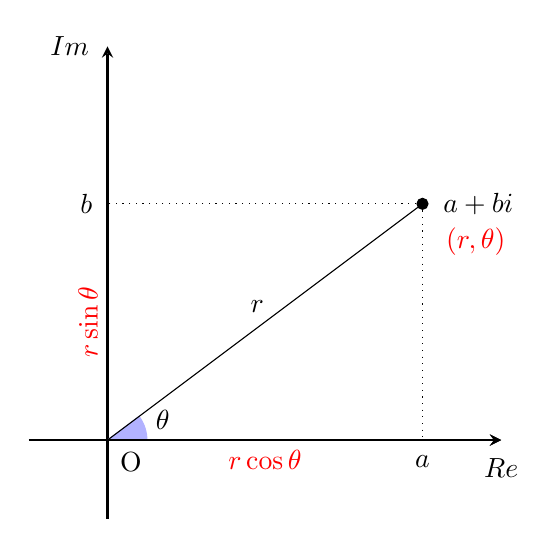
\begin{tikzpicture}
            \pgfmathsetmacro{\axislimit}{5}

            \node[below right=1pt] (origin) at (0,0) {\(\rm{O}\)};
            \draw [-stealth,thick] (-1, 0) -- (\axislimit, 0) node[below=3pt] {\(\mf{Re}\)};
            \draw [-stealth,thick] (0, -1) -- (0, \axislimit) node[left=3pt] {\(\mf{Im}\)};

            \onslide<2->{
                \coordinate (point) at (4, 3);
                \filldraw[fill=black] (point) circle (0.07);
                \node [right=4pt] at (point) {\(a + bi\)};
                \draw [dotted] (point) -- (4, 0);
                \draw [dotted] (point) -- (0, 3);

                \node [below=2pt] at (4, 0) {\(a\)};
                \node [left=2pt] at (0, 3) {\(b\)};
            }

            \onslide<3-> {
                \filldraw[color=blue!30] (0.5, 0) arc (0:36.869:0.5) -- (0, 0);
                \draw (0, 0) -- (point);
                \draw [-stealth,thick] (-1, 0) -- (\axislimit, 0);
                \node at (0.7, 0.25) {\(\theta\)};
                \node at (1.9, 1.7) {\(r\)};
            }

            \onslide<4-> {
                \node [below right=5pt, color=red] at (point) {\((r, \theta)\)};
                \node [below, color=red] at (2, 0) {\(r\cos\theta\)};
                \node [above, color=red, rotate=90] at (0, 1.5) {\(r\sin\theta\)};
            }
        \end{tikzpicture}
    \end{center}
\end{frame}


\begin{frame}
    \frametitle{복소수의 극형식}
    \begin{itemize}
        \item \alert{극형식}(polar form): \(z = (r, \theta) = r(\cos\theta + i\sin\theta)\) \pause
              \medskip
              \begin{itemize}
                  \item \(r = \abs{z} = \sqrt{a^2 + b^2}\) (원점과의 거리)
                        \medskip
                  \item \(\theta = \arg{z}\) (실수 축의 양의 방향과 이루는 각) \pause
              \end{itemize}
              \medskip
        \item 곱셈
              \[
                  (r_1, \theta_1) \cdot (r_2, \theta_2) = (r_1 r_2, \theta_1 + \theta_2)
              \]
        \item 나눗셈
              \[
                  \frac{(r_1, \theta_1)}{(r_2, \theta_2)} = \left(\frac{r_1}{r_2}, \theta_1 - \theta_2\right)
              \] \pause
        \item 손쉬워진 곱셈과 나눗셈!
    \end{itemize}
\end{frame}

\subsection*{Roots of Unity}
\begin{frame}
    \frametitle{Roots of Unity}
    \begin{theorem}[드 무아브르의 정리]
        복소수 \(z = (r, \theta)\)\,에 대하여,
        \begin{center}
            \(z^n = (r, \theta)^n = (r^n, n\theta)\)
        \end{center}
    \end{theorem}

    \pause

    \begin{itemize}
        \item \(n\)\,제곱 하면 거리는 \(n\)\,제곱 되고 각은 \(n\)\,배가 된다. \pause
        \item \alert{방정식 \(z^n = 1\) 의 해는?}
    \end{itemize}
\end{frame}

\begin{frame}
    \frametitle{Roots of Unity}
    \begin{itemize}
        \setlength{\itemsep}{1em}
        \item \(z = (r, \theta)\)\,라고 하면, \(z^n = (r^n, n\theta)\). \pause
        \item \(1 = (1, 2k\pi)\)\,이므로 (\(k\): 정수)
              \vspace*{10px}
              \begin{center}
                  \(r^n = 1\) and \(n\theta = 2k\pi\)
              \end{center} \pause
        \item \(r \geq 0\)\,이고 \(z^n = 1\)\,은 정확히 \(n\)\,개의 해를 가지므로,
              \vspace*{10px}
              \begin{center}
                  \alert{\(r = 1\)} and \alert{\(\ds \theta = \frac{2k\pi}{n}\)} \quad \((k = 0, \dots, n - 1)\)
              \end{center} \pause
        \item 이 \(n\)\,개의 해를 \alert{roots of unity}\,라 하고 \(\ds \omega_n = \left(1, \frac{2\pi}{n}\right)\)\,으로 표기
    \end{itemize}
\end{frame}

\begin{frame}
    \frametitle{예: \(z^7 = 1\) 의 해}
    \begin{center}
        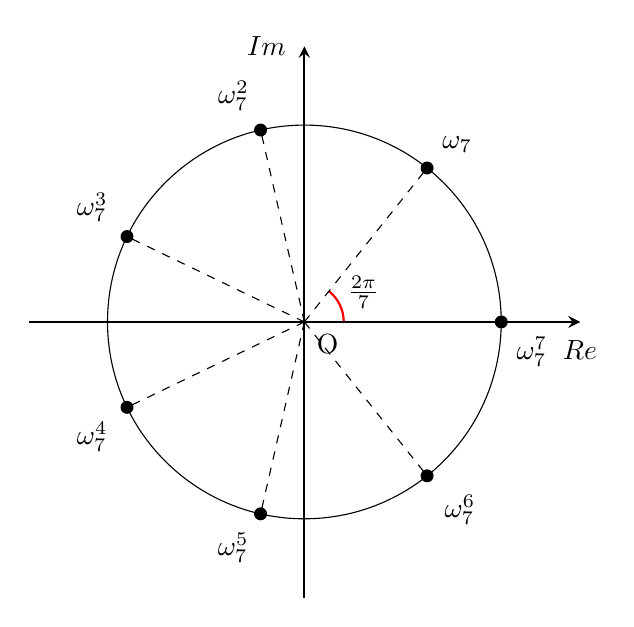
\begin{tikzpicture}[scale=2.5]
            \pgfmathsetmacro{\axislimit}{1.4}

            \node[below right=1pt] (origin) at (0,0) {\(\rm{O}\)};
            \draw [-stealth,thick] (-\axislimit, 0) -- (\axislimit, 0) node[below=3pt] {\(\mf{Re}\)};
            \draw [-stealth,thick] (0, -\axislimit) -- (0, \axislimit) node[left=3pt] {\(\mf{Im}\)};

            \coordinate (one) at (1, 0);
            \filldraw[fill=black] (one) circle (0.03) node[below right=2pt] {\(1\)};

            \onslide<2->{
                \coordinate (omega1) at (360/7:1);
                \filldraw[fill=black] (omega1) circle (0.03) node[above right=2pt] {\(\omega_7\)};
                \draw[color=red,thick] (0.2, 0) arc (0:360/7:0.2);
                \node at (0.3, 0.15) {\(\frac{2\pi}{7}\)};
                \draw[dashed] (0, 0) -- (omega1);
                \draw [-stealth,thick] (-\axislimit, 0) -- (\axislimit, 0);
            }

            \onslide<3-> {
                \draw (0, 0) circle (1);
            }

            \onslide<4->{
                \foreach \k in {2, 3, 4, 5, 6} {
                        \filldraw[fill=black] (360/7 * \k:1) circle (0.03);
                        \node[label=360/7 * \k:\(\omega_7^{\k}\)] at (360/7 * \k:1) {};
                        \draw[dashed] (0, 0) -- (360/7 * \k:1);
                    }

                \node[below right=2pt, fill=white] at (1, 0) {\(\omega_7^7\)};
            }
        \end{tikzpicture}
    \end{center}
\end{frame}

\begin{frame}
    \frametitle{\(\omega_n\) 의 성질}

    % n제곱 해야 1, 그 전엔 절대 1 아님
    % 또 FFT 증명에 사용되는 성질 하나 넣기

    \begin{columns}
        \column{0.5\textwidth}
        \begin{itemize}
            \item \(\omega_n^k \neq 1\) for \(1 \leq k \leq n - 1\)
                  \medskip
            \item \alert{\(\omega_n^n = 1\)}
                  \medskip
            \item<2->{짝수 \(n\)에 대하여,
                  \medskip
                  \begin{itemize}
                      \item \alert{\(\omega_n^{n/2} = -1\)}
                            \medskip
                      \item \(\omega_n^{\alert{2}} = \omega_{n/\alert{2}}\)
                  \end{itemize}}
        \end{itemize}

        \column{0.55\textwidth}
        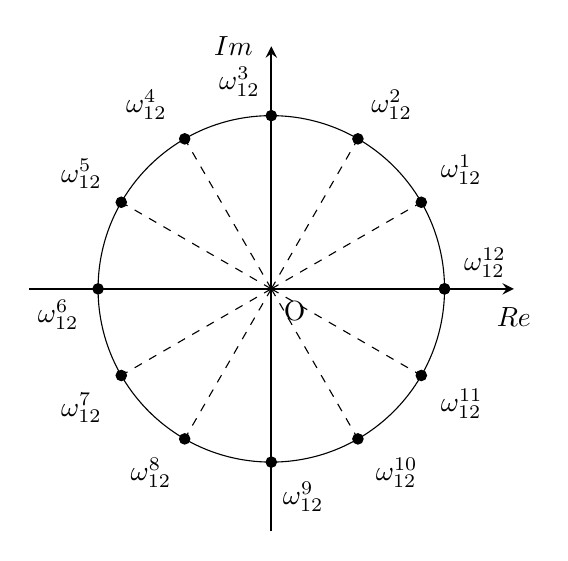
\begin{tikzpicture}[scale=2.2]
            \pgfmathsetmacro{\axislimit}{1.4}
            \pgfmathsetmacro{\n}{12}
            \node[below right=1pt] (origin) at (0,0) {\(\rm{O}\)};
            \draw [-stealth,thick] (-\axislimit, 0) -- (\axislimit, 0) node[below=3pt] {\(\mf{Re}\)};
            \draw [-stealth,thick] (0, -\axislimit) -- (0, \axislimit) node[left=3pt] {\(\mf{Im}\)};

            \coordinate (one) at (1, 0);
            \filldraw[fill=black] (one) circle (0.03);
            \draw (0, 0) circle (1);

            \foreach \k in {1, ..., \n} {
                    \filldraw[fill=black] (360/\n * \k:1) circle (0.03);
                    \node[label=360/\n * \k + 10:\(\omega_{\n}^{\k}\)] at (360/\n * \k:1) {};
                    \draw[dashed] (0, 0) -- (360/\n * \k:1);
                }
        \end{tikzpicture}
    \end{columns}
\end{frame}

\begin{frame}
    \begin{center}

        \begin{tikzpicture}[scale=2.5]
            \pgfmathsetmacro{\axislimit}{1.4}
            \pgfmathsetmacro{\n}{12}
            \node[color=white,label={30:\(\color{white} {\omega_{6}^6} = \omega_{12}^{12}\)}] at (360:1) {};
            \node[below right=1pt] (origin) at (0,0) {\(\rm{O}\)};
            \draw [-stealth,thick] (-\axislimit, 0) -- (\axislimit, 0) node[below=3pt] {\(\mf{Re}\)};
            \draw [-stealth,thick] (0, -\axislimit) -- (0, \axislimit) node[left=3pt] {\(\mf{Im}\)};
            \coordinate (one) at (1, 0);
            \draw (0, 0) circle (1);

            \only<1> {
                \filldraw[fill=black] (one) circle (0.03);
                \foreach \k in {1, ..., \n} {
                        \filldraw[fill=black] (360/\n * \k:1) circle (0.03);
                        \node[label=360/\n * \k + 10:\(\omega_{\n}^{\k}\)] at (360/\n * \k:1) {};
                        \draw[dashed] (0, 0) -- (360/\n * \k:1);
                    }
            }

            \only<2-> {
                \foreach \k in {1, ..., \n} {
                        \filldraw[fill=black] (360/\n * \k:1) circle (0.03);
                    }
                \draw[-stealth,thick,color=red] (35:1.15) arc (35:55:1.15);
                \node[label=0:\(\omega_{\n}\)] at (360/\n:1) {};

                \draw[-stealth,thick,color=red] (95:1.15) arc (95:175:1.15);
                \node[label=45:\(\omega_{\n}^3\)] at (360/\n * 3:1) {};

                \draw[-stealth,thick,color=red] (185:1.15) arc (185:355:1.15);
                \node[label=-45:\(\omega_{\n}^6\)] at (360/\n * 6:1) {};
            }

            \only<3> {
                \foreach \k in {1, ..., 6} {
                        \filldraw[fill=red] (60 * \k:1) circle (0.03);
                        \draw[color=red,dashed] (0, 0) -- (60 * \k:1);
                    }

                \node[color=red,label={80:\({\color{red}\omega_{6}} = \omega_{12}^2\)}] at (60:1) {};
                \node[color=red,label={30:\({\color{red}\omega_{6}^3} = \omega_{12}^6\)}] at (180:1) {};
                \node[color=red,label={30:\({\color{red}\omega_{6}^6} = \omega_{12}^{12}\)}] at (360:1) {};
            }
        \end{tikzpicture}
    \end{center}
\end{frame}

\subsection*{다항식}

\begin{frame}
    \frametitle{다항식}
    \begin{itemize}
        \setlength{\itemsep}{1em}
        \item \(R[x]\): Ring \(R\)\,의 원소를 계수로 갖는 다항식의 집합
              \smallskip
              \begin{itemize}
                  \item \(\R[x]\): 실수 계수 다항식의 집합
                        \smallskip
                  \item \(\Z_n[x]\): 정수 계수 다항식의 집합 (단, 계수는 모두 \(\rm{mod} \; n\))
              \end{itemize}

        \item<2-> 벡터로도 표기\footnote<2->{어차피 \(x\)는 symbol일 뿐...}
              \smallskip
              \begin{itemize}
                  \item \(f(x) = \ds \sum_{i=0}^{n-1} a_{i}x^i = a_0 + a_1x + a_2x^2 + \cdots + a_{n-1}x^{n-1}\)
                        \smallskip
                  \item \(f = \left(a_0, a_1, \dots, a_{n-1}\right)\)
              \end{itemize}

        \item<3-> 다항식 \(f(x)\)\,의 차수를 \(\deg f\)\,로 나타냄
        \item<4-> \(\Z_{10001}\)\,에서 \(x^2 - 1 = (x - 2191)(x - 7810)\) (!)
    \end{itemize}
\end{frame}

\subsection*{합동식}

\begin{frame}
    \frametitle{합동식}
    \begin{itemize}
        \setlength{\itemsep}{2em}
        \item 정수 \(a\)를 정수 \(b\)로 나눈 몫과 나머지가 각각 \(q,\,r\)일 때,
              \smallskip
              \begin{center}
                  \(a = bq + r\) \quad and \quad \(a \equiv r \pmod{b}\)
              \end{center}
              \smallskip
              \begin{itemize}
                  \item 프로그래밍 언어들에 존재하는 \textsc{\%} 연산
                        \medskip
                  \item \(17 \equiv 4 \pmod{13}\)
              \end{itemize}
        \item<2-> 다항식 \(A\)를 다항식 \(B\)로 나눈 몫과 나머지가 각각 \(Q,\,R\)일 때,
              \smallskip
              \begin{center}
                  \(A = BQ + R\) \quad and \quad \(A \equiv R \pmod{B}\)
              \end{center}
              \smallskip
              \begin{itemize}
                  \item<3-> \(x^2 + 5x + 4 = (x + 2)^2 + x\)
                        \medskip
                  \item<3-> \(x^2 + 5x + 4 \equiv x \pmod{(x + 2)^2}\)
              \end{itemize}
    \end{itemize}
\end{frame}

\section{다항식의 연산}

\subsection{덧셈 in \texorpdfstring{\(\O(n)\)}{O(n)}}

\begin{frame}[fragile]
    \frametitle{다항식의 덧셈}
    \begin{itemize}
        \setlength{\itemsep}{1em}
        \item Very easy!
        \item<2-> \(f = (a_0, \dots, a_{n-1})\), \(g = (b_0, \dots, b_{n-1})\)
              \smallskip
              \begin{center}
                  \(f + g = (a_0 + b_0, \dots, a_{n-1} + b_{n-1})\)
              \end{center}
        \item<2-> 당연히 \(\O(n)\)!
        \item<3->
              \begin{center}
                  \begin{lstlisting}[language=Python]
  def add(f: List[int], g: List[int]) -> List[int]:
      return [f[i] + g[i] for i in range(len(f))]
\end{lstlisting}
              \end{center}
    \end{itemize}
\end{frame}

\subsection{곱셈 in \texorpdfstring{\(\O(n^2)\)}{O(n2)}}

\begin{frame}
    \frametitle{다항식의 곱셈}
    \begin{itemize}
        \setlength{\itemsep}{1em}
        \item<2-> \(\ds f = \sum_{i = 0}^{n - 1} a_i x^i\), \(\ds g = \sum_{i = 0}^{n - 1} b_i x^i\),
              \smallskip
              \begin{center}
                  \(\ds fg = \sum_{i = 0}^{2n - 1} \sum_{j = 0}^{i} a_{j} b_{i - j} x^i\)
              \end{center}
              \begin{itemize}
                  \item<3-> \(i\)\,는 \alert{차수}를 나타냄
                        \medskip
                  \item<4-> \(x^i\)\,의 계수: \(0 \leq j \leq i\)\,에 대하여 \(a_j\)\,와 \(b_{i-j}\)\,를 곱해 더한 것
                        \medskip
                  \item<4-> \(a_j x^j \cdot b_{i - j} x^{i - j} = \alert{a_j b_{i-j}} x^{i}\)
              \end{itemize}
        \item<5-> \(\sum\)\,가 두 개 들어간 것을 보니 \(\O(n^2)\)\,...
        \item<6-> \textit{어디서 많이 본 것 같은데...}
    \end{itemize}
\end{frame}

\begin{frame}[fragile]
    \frametitle{다항식의 곱셈}
    \begin{center}
        \begin{lstlisting}[language=Python]
    def multiply(f: List[int], g: List[int]) -> List[int]:
        product = [0] * (len(f) + len(g))

        for i in range(len(product)):
            for j in range(i + 1):
                product[i] += f[i] * g[j - i]

        return product
\end{lstlisting}
    \end{center}
\end{frame}

\section{이산 푸리에 변환 (DFT)}

\begin{frame}
    \frametitle{합성곱}
    \begin{block}{\textbf{합성곱(Convolution)}}
        두 벡터 \(\mathbf{a} = \left(a_0,\,\dots,\,a_{n-1}\right)\), \(\mathbf{b} = \left(b_0,\,\dots,\,b_{n-1}\right)\)\,에 대하여 이들의 \alert{합성곱} \(\mathbf{c} = \mathbf{a} \ast \mathbf{b}\)\,를
        \[
            c_i = \sum_{j = 0}^{i} \alert{a_{j} b_{i - j}} \qquad (i = 0,\,1\,\dots\,2n - 1)
        \]
        과 같이 정의한다.
    \end{block}

    \pause

    \begin{itemize}
        \item<2-> 다항식의 곱 형태와 동일한 모양: \alert{\(fg = f \ast g\)}
        \item<3-> 여전히 계산에는 \(\O(n^2)\)\,이 걸림
        \item<4-> Convolution\,을 빠르게... \textit{Fast Fourier Transform}?
    \end{itemize}
\end{frame}

\subsection{DFT}

\begin{frame}
    \frametitle{이산 푸리에 변환}
    \begin{block}{\textbf{Discrete Fourier Transform}}
        다항식 \(f = \left(a_0,\,\dots,\,a_{n-1}\right)\)\,의 \alert{이산 푸리에 변환}(DFT)을 다음과 같이 정의한다.
        \[
            \DFT(f) = \big(f(1),\, f(\omega),\, f(\omega^2),\, \dots\, f(\omega^{n-1})\big)
        \]
        단, \(\omega = \omega_n\) 이다.
    \end{block}

    \pause

    \begin{itemize}
        \item<2-> Roots of unity\,에 대해 \(f\)\,의 함숫값을 계산한 결과
        \item<3-> 결과는 \alert{벡터}
    \end{itemize}
\end{frame}

\begin{frame}
    \begin{theorem}
        다항식 \(f,\, g\)\,에 대하여 다음이 성립한다.
        \vspace*{-5px}
        \[
            \alert{\DFT(f \ast g) = \DFT(f) \cdot \DFT(g)}
        \]
        \vspace*{-15px}
    \end{theorem}

    \begin{itemize}
        \setlength{\itemsep}{1em}
        \item<2-> 우변의 \(\cdot\)\,은 성분별 곱 (component-wise product)
        \item<3-> \(f,\,g\)\,가 \(n\)\,차 다항식이면 \(fg\)\,는 \(2n\)\,차 다항식
        \item<4-> \(f,\,g\)\,를 \(2n\)\,차 다항식으로 간주하고 DFT\,를 계산
        \item<4-> \(f = (a_0,\,\dots,\,a_{n-1},\, \underbrace{0,\, \dots,\, 0}_{n\,\text{개}})\)
    \end{itemize}
\end{frame}


\begin{frame}
    \begin{proof}
        각 변의 \(k\)\,번째 성분만 비교하면 충분하다.
        \begin{center}
            (좌변) \(= (f \ast g)(\omega_{2n}^k) = (fg)(\omega_{2n}^k) = f(\omega_{2n}^k)g(\omega_{2n}^k) = \) (우변)
        \end{center}
    \end{proof}

    \pause

    \begin{corollary}
        다항식 \(f,\, g\)\,에 대하여 다음이 성립한다.
        \vspace*{-5px}
        \[
            \alert{f \ast g = \DFT\inv\left(\DFT(f) \cdot \DFT(g)\right)}
        \]
        \vspace*{-15px}
    \end{corollary}
\end{frame}

\subsection{Inverse DFT}

\begin{frame}
    \frametitle{DFT Matrix}
    \(\DFT(f)\)\,는 다음과 같이 표현 가능
    \[
        \DFT(f) = \underbrace{\begin{bmatrix}
                1      & 1              & 1                 & \cdots & 1                       \\
                1      & \omega         & \omega^2          & \cdots & \omega^{n - 1}          \\
                1      & \omega^2       & \omega^4          & \cdots & \omega^{2(n - 1)}       \\
                \vdots & \vdots         & \vdots            & \ddots & \vdots                  \\
                1      & \omega^{n - 1} & \omega^{2(n - 1)} & \cdots & \omega^{(n - 1)(n - 1)}
            \end{bmatrix}}_{W}
        \begin{bmatrix}
            a_0 \\ a_1 \\ a_2 \\ \vdots \\ a_{n - 1}
        \end{bmatrix} =
        \begin{bmatrix}
            f(1) \\ f(\omega) \\ f(\omega^2) \\ \vdots \\ f(\omega^{n - 1})
        \end{bmatrix}
    \]

    \pause

    \begin{itemize}
        \item<2-> \alert{DFT 행렬}: \(\ds W = \left(\omega^{ij}\right)_{n \times n}\) (0-based index)
        \item<3-> 역행렬만 찾아서 곱하면 Inverse DFT!
    \end{itemize}
\end{frame}

\begin{frame}
    \frametitle{DFT Matrix}
    \begin{theorem}
        DFT 행렬의 역행렬 \(W\inv\)\,는 다음과 같다.
        \[
            W\inv = \left(\frac{\omega^{-ij}}{n}\right)_{n\times n} = \frac{1}{n}\begin{bmatrix}
                1      & 1                 & 1                  & \cdots & 1                        \\
                1      & \omega^{-1}       & \omega^{-2}        & \cdots & \omega^{-(n - 1)}        \\
                1      & \omega^{-2}       & \omega^{-4}        & \cdots & \omega^{-2(n - 1)}       \\
                \vdots & \vdots            & \vdots             & \ddots & \vdots                   \\
                1      & \omega^{-(n - 1)} & \omega^{-2(n - 1)} & \cdots & \omega^{-(n - 1)(n - 1)}
            \end{bmatrix}
        \]
    \end{theorem}

    \pause

    \begin{proof}
        곱해보시라!
    \end{proof}
\end{frame}

\begin{frame}
    \frametitle{Inverse DFT}

    따라서, \(f = \DFT\inv(\DFT(f)) = W\inv \begin{bmatrix} f(1) \\ f(\omega) \\ \vdots \\ f(\omega^{n - 1}) \end{bmatrix}\)

    \pause
    \begin{theorem}
        다항식 \(f\)\,에 대하여 \(g = \DFT(f)\)\,라 하자. 그러면
        \[
            f = \DFT\inv(g) = \big(g(1),\, g(\omega^{-1}),\, g(\omega^{-2}),\, \dots,\, g(\omega^{-(n-1)})\big)
        \]
        이다.
    \end{theorem}
\end{frame}

\begin{frame}
    \frametitle{\(\DFT\) vs \(\DFT\inv\)}

    임의의 벡터 \((a_0,\, a_1,\, \dots,\, a_{n - 1})\)\,에 대하여 이를 다항식처럼 간주하고

    roots of unity\,에 대해
    \begin{columns}
        \column{0.5\textwidth}

        \begin{itemize}
            \item<2-> \(\DFT\): \alert{반시계} 방향으로 계산
        \end{itemize}
        \begin{center}
            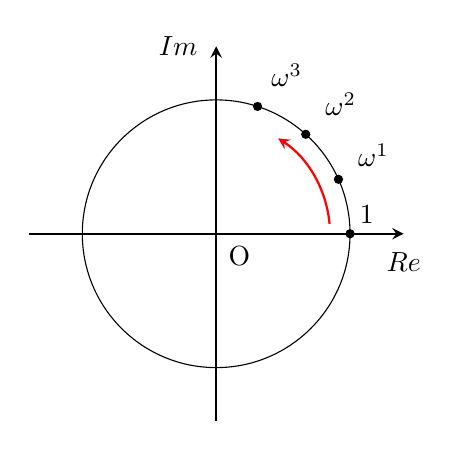
\begin{tikzpicture}[scale=1.7]
                \pgfmathsetmacro{\axislimit}{1.4}
                \pgfmathsetmacro{\n}{15}
                \node[below right=1pt] (origin) at (0,0) {\(\rm{O}\)};
                \draw [-stealth,thick] (-\axislimit, 0) -- (\axislimit, 0) node[below=3pt] {\(\mf{Re}\)};
                \draw [-stealth,thick] (0, -\axislimit) -- (0, \axislimit) node[left=3pt] {\(\mf{Im}\)};
                \draw (0, 0) circle (1);

                \only<2->{
                    \coordinate (one) at (1, 0);
                    \filldraw[fill=black] (one) circle (0.03) node[above right] {\(1\)};

                    \foreach \k in {1, 2, 3} {
                            \filldraw[fill=black] (360/\n * \k:1) circle (0.03);
                            \node[label=360/\n * \k - 5:\(\omega^{\k}\)] at (360/\n * \k:1) {};
                        }

                    \draw[-stealth,thick,color=red] (5:0.85) arc (5:57:0.85);
                }
            \end{tikzpicture}
        \end{center}

        \column{0.5\textwidth}
        \begin{itemize}
            \item<3-> \(\DFT\inv\): \alert{시계} 방향으로 계산
        \end{itemize}
        \begin{center}
            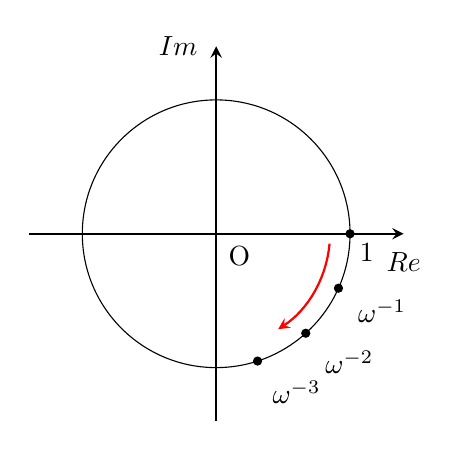
\begin{tikzpicture}[scale=1.7]
                \pgfmathsetmacro{\axislimit}{1.4}
                \pgfmathsetmacro{\n}{15}
                \node[below right=1pt] (origin) at (0,0) {\(\rm{O}\)};
                \draw [-stealth,thick] (-\axislimit, 0) -- (\axislimit, 0) node[below=3pt] {\(\mf{Re}\)};
                \draw [-stealth,thick] (0, -\axislimit) -- (0, \axislimit) node[left=3pt] {\(\mf{Im}\)};
                \draw (0, 0) circle (1);

                \only<3->{
                \coordinate (one) at (1, 0);
                \filldraw[fill=black] (one) circle (0.03) node[below right] {\(1\)};

                \foreach \k in {1, 2, 3} {
                        \filldraw[fill=black] (-360/\n * \k:1) circle (0.03);
                        \node[label=-360/\n * \k + 10:\(\omega^{-\k}\)] at (-360/\n * \k:1) {};
                    }

                \draw[-stealth,thick,color=red] (-5:0.85) arc (-5:-57:0.85);
                }
            \end{tikzpicture}
        \end{center}
    \end{columns}
\end{frame}

\section{고속 푸리에 변환 (FFT)}

\begin{frame}
    \frametitle{고속 푸리에 변환}
    \begin{itemize}
        \setlength{\itemsep}{1em}
        \item DFT\,는 그냥 계산하면 \(\O(n^2)\)\,이 소요됨 \pause
        \item \(\omega_n^2 = \omega_{n/2}\) \(\rightarrow\) 분할 정복을 시도!
    \end{itemize}
\end{frame}

\begin{frame}
    \frametitle{고속 푸리에 변환}
    이 절에서는 \(n = 2^k\) (\(k\): 정수) 임을 가정합니다.

    \pause

    \begin{block}{\textbf{Fast Fourier Transform}}
        \(f(x) = a_0 + a_1 x + a_2 x^2 + \cdots + a_{n-1} x^{n - 1}\)\,에 대하여
        \begin{itemize}
            \item \alert{짝수} 차수 항의 계수를 모은 다항식
                  \vspace*{-10px}
                  \[
                      f_{\mathrm{even}} = a_0 + a_2 x + a_4 x^2 + \cdots + a_{n-2} x^{n/2 - 1}
                  \]
                  \vspace*{-30px}
            \item \alert{홀수} 차수 항의 계수를 모은 다항식
                  \vspace*{-10px}
                  \[
                      f_{\mathrm{odd}} = a_1 + a_3 x + a_5 x^2 + \cdots + a_{n-1} x^{n/2 - 1}
                  \]
                  \vspace*{-20px}
        \end{itemize}
        을 생각합니다. \pause 그러면 다음이 성립합니다.
        \vspace*{-5px}
        \begin{center}
            \alert{\(f(x) = f_{\mathrm{even}}(x^2) + x f_{\mathrm{odd}}(x^2)\)}
        \end{center}
        \vspace*{3px}
    \end{block}
\end{frame}

\begin{frame}
    \begin{block}{\textbf{Fast Fourier Transform} (continued)}
        \(\DFT(f)\)\,를 계산하려면, \(f(\omega_{n}^i)\)\,를 계산해야 합니다.
        \[
            f(\omega_{n}^i) = f_{\mathrm{even}}(\omega_{n}^{\alert{2}i}) + \omega_n^i f_{\mathrm{odd}}(\omega_{n}^{\alert{2}i})
        \]
        이고, \pause \(\omega_n^{\alert{2}} = \omega_{n/\alert{2}}\) 이므로
        \[
            f(\omega_{n}^i) = f_{\mathrm{even}}(\omega_{n/\alert{2}}^{i}) + \omega_n^i f_{\mathrm{odd}}(\omega_{n/\alert{2}}^{i})
        \]
        입니다. \pause 한편 \(i = 0,\, 1,\, \dots,\, n - 1\) 인데,
        \[\omega_{n/2}^{i + n/2} = \omega_{n/2}^i \cdot \omega_{n/2}^{n/2} = \omega_{n/2}^i\]
        이므로 사실상 \alert{절반이 겹칩니다!}
    \end{block}
\end{frame}

\begin{frame}
    \begin{block}{\textbf{Fast Fourier Transform} (continued)}
        결국 \(\DFT(f)\)\,를 계산하기 위해서는 \pause
        \begin{itemize}
            \item \(\DFT(f_{\mathrm{even}})\) 계산 \pause
            \item \(\DFT(f_{\mathrm{odd}})\) 계산 \pause
            \item 계산 결과 합치기
        \end{itemize}
        의 과정으로 충분합니다.

        \pause

        \vspace*{10px}

        그런데 \(f_{\mathrm{even}}\), \(f_{\mathrm{odd}}\)\,는 항이 \alert{\(n/2\)}\,개 이므로 이 알고리즘의 시간 복잡도는
        \[
            T(n) = 2T\left(\frac{n}{2}\right) + \O(n) \implies T(n) \in \alert{\O(n\log n)}
        \]
        입니다.
    \end{block}
\end{frame}

\begin{frame}[fragile]
    \frametitle{FFT 구현} \small
    \[
        f(\omega_n^{i}) = \begin{cases}
            f_{\mathrm{even}}(\omega_{n/2}^i) + \omega_{n}^i f_{\mathrm{odd}}(\omega_{n/2}^i) & \text{for } i = 0,\, 1,\, \dots,\, \dfrac{n}{2} \\
            f_{\mathrm{even}}(\omega_{n/2}^i) - \omega_{n}^i f_{\mathrm{odd}}(\omega_{n/2}^i) & \text{for } i = \dfrac{n}{2},\, \dots,\, n - 1
        \end{cases}
    \]

    \begin{lstlisting}[language=Python]
    # Assuming len(f) is a power of 2
    def fft(f: List[complex]) -> List[complex]:
        n = len(f)
        if n <= 1:
            return f

        f_even, f_odd = f[::2], f[1::2]
        fft_even, fft_odd = fft(f_even), fft(f_odd)

        result = [0] * n
        for i in range(n // 2):
            omega = complex(cos(2 * pi / n), sin(2 * pi / n)) ** i

            result[i] = fft_even[i] + omega * fft_odd[i]
            result[i + n // 2] = fft_even[i] - omega * fft_odd[i]

        return result
\end{lstlisting}
\end{frame}

\begin{frame}[fragile]
    \frametitle{Inverse FFT 구현} \small
    Inverse FFT 또한 \(\O(n \log n)\)\,에 수행 가능:
    \begin{itemize}
        \item \(\omega_n^i\)\,만 \(\omega_n^{-i}\)\,로 바뀜
        \item 마지막에 \(1/n\) 해줘야 함
    \end{itemize}

    \begin{lstlisting}[language=Python]
    # Assuming len(f) is a power of 2
    def inverse_fft(f: List[complex]) -> List[complex]:
        n = len(f)
        if n <= 1:
            return f

        f_even, f_odd = f[::2], f[1::2]
        inverse_fft_even, inverse_fft_odd = inverse_fft(f_even), inverse_fft(f_odd)

        result = [0] * n
        for i in range(n // 2):
            omega = complex(cos(2 * pi / n), sin(2 * pi / n)) ** -i

            result[i] = inverse_fft_even[i] + omega * inverse_fft_odd[i]
            result[i + n // 2] = inverse_fft_even[i] - omega * inverse_fft_odd[i]

        return [result_i / 2 for result_i in result]
\end{lstlisting}
\end{frame}

\subsection{곱셈 in \texorpdfstring{\(\O(n \log n)\)}{O(nlogn)}}

\begin{frame}
    \frametitle{다항식의 곱셈 in \(\O(n\log n)\)}
    \begin{center}
        \begin{tikzpicture}[scale=0.6]
            \node (f and g) at (-6, 4) {\(f,\, g\)};
            \node (fg) at (6, 4) {\(fg\)};

            \draw[white,->,thick] (f and g) -- (fg) node[midway,above] {direct multiplication} node[midway,below] {\(\O(n^2)\)};
            \node[white] (dft) at (-6, -4) {\(\DFT(f),\, \DFT(g)\)};
            \draw[white,->,thick] (f and g) -- (dft) node[midway,left] {\(\DFT\)} node[midway,right] {\(\O(n\log n)\)};
            \node[white] (dftf_dftg) at (6, -4) {\(\DFT(f)\cdot\DFT(g)\)};
            \draw[white,->,thick] (dft) -- (dftf_dftg) node[midway,below] {dot product} node[midway,above] {\(\O(n)\)};
            \draw[white,->,thick] (dftf_dftg) -- (fg) node[midway,right] {\(\DFT\inv\)} node[midway,left] {\(\O(n\log n)\)};

            \only<2->{
                \draw[->,thick] (f and g) -- (fg) node[midway,above] {direct multiplication} node[midway,below] {\(\O(n^2)\)};
            }

            \only<3->{
                \node (dft) at (-6, -4) {\(\DFT(f),\, \DFT(g)\)};
                \draw[->,thick,red] (f and g) -- (dft) node[midway,left] {\(\DFT\)} node[midway,right] {\(\O(n\log n)\)};
            }

            \only<4->{
                \node (dftf_dftg) at (6, -4) {\(\DFT(f)\cdot\DFT(g)\)};
                \draw[->,thick,red] (dft) -- (dftf_dftg) node[midway,below] {dot product} node[midway,above] {\(\O(n)\)};
            }

            \only<5->{
                \draw[->,thick,red] (dftf_dftg) -- (fg) node[midway,right] {\(\DFT\inv\)} node[midway,left] {\(\O(n\log n)\)};
            }
        \end{tikzpicture}
    \end{center}
\end{frame}

\subsection{나눗셈 in \texorpdfstring{\(\O(n \log n)\)}{O(nlogn)}}

\begin{frame}
    \frametitle{다항식의 나눗셈 in \(\O(n\log n)\)}
    \begin{itemize}
        \item<1-> \textit{나눗셈은 역수의 곱셉!} \pause \alert{이라고 할 뻔!}\footnote<2->{Ring\,은 나눗셈을 보장하지 않습니다}
    \end{itemize}

    \pause

    \begin{block}{다항식의 나눗셈}
        다항식 \(A(x)\), \(B(x)\)\,에 대하여
        \[
            A(x) = B(x)Q(x) + R(x)
        \]
        인 다항식 \(Q(x)\)\,와 \(\deg R < \deg B\)\,인 다항식 \(R(x)\)\,가 유일하게 존재한다.

        이 때 \(Q(x)\)\,를 \alert{몫}, \(R(x)\)\,를 \alert{나머지}라고 한다.
    \end{block}
\end{frame}

\begin{frame}
    \begin{itemize}
        \setlength{\itemsep}{0.8em}
        \item \(\deg A = n\), \(\deg B = m\)\,이라 하면 \(\deg Q = n - m\)\,이므로 \pause
              \begin{itemize}
                  \item \(A(x) = a_0 + a_1 x + a_2 x^2 + \cdots + a_{n} x^{n}\)
                  \item \(B(x) = b_0 + b_1 x + b_2 x^2 + \cdots + b_{m} x^{m}\)
                  \item \(Q(x) = q_0 + q_1 x + q_2 x^2 + \cdots + q_{n - m} x^{n - m}\)
              \end{itemize}
              \pause
        \item 어차피 \(R(x)\)\,의 차수는 \(m = \deg B\)\,를 넘지 않으므로 \(A(x)\)\,의 첫 \(n - m + 1\)\,개의 항에 영향을 줄 수 없음 \pause
        \item \(A = BQ + R\)\,에서 양변의 첫 \(n - m + 1\)개 항 계수를 비교
              \[
                  \begin{bmatrix}
                      a_n \\ a_{n - 1} \\ \vdots \\ a_{m + 1} \\ a_m
                  \end{bmatrix} = \begin{bmatrix}
                      b_m       & 0      & \cdots & 0         & 0      \\
                      b_{m - 1} & b_m    & \cdots & 0         & 0      \\
                      \vdots    & \vdots & \ddots & \vdots    & \vdots \\
                      \ast      & \ast   & \cdots & b_m       & 0      \\
                      \ast      & \ast   & \cdots & b_{m - 1} & b_m
                  \end{bmatrix} \begin{bmatrix}
                      q_{n - m} \\ q_{n - m - 1} \\ \vdots \\ q_1 \\ q_0
                  \end{bmatrix}
              \]
    \end{itemize}
\end{frame}

\begin{frame}
    \[\small
        \begin{bmatrix}
            a_n \\ a_{n - 1} \\ \vdots \\ a_{m + 1} \\ a_m
        \end{bmatrix} = \begin{bmatrix}
            b_m       & 0      & \cdots & 0         & 0      \\
            b_{m - 1} & b_m    & \cdots & 0         & 0      \\
            \vdots    & \vdots & \ddots & \vdots    & \vdots \\
            \ast      & \ast   & \cdots & b_m       & 0      \\
            \ast      & \ast   & \cdots & b_{m - 1} & b_m
        \end{bmatrix} \begin{bmatrix}
            q_{n - m} \\ q_{n - m - 1} \\ \vdots \\ q_1 \\ q_0
        \end{bmatrix}
    \]
    \begin{itemize}
        \setlength{\itemsep}{0.8em}
        \item 구하는 것은 \(Q(x)\)\,이므로 역행렬을 계산해도 되지만...
        \item<2-> Reversed Polynomial\,을 도입 (다항식 계수 뒤집기!)
              \begin{itemize}
                  \item \(A_R(x) = x^n A(x\inv) = a_n + a_{n - 1} x + \cdots + a_0 x^n\)
                  \item \(B_R(x) = x^m B(x\inv) = b_m + b_{m - 1} x + \cdots + b_0 x^m\)
                  \item \(Q_R(x) = x^{n - m} Q(x\inv) = q_{n - m} + q_{n - m - 1} x + \cdots + q_0 x^{n - m}\)
              \end{itemize} \pause
        \item<4-> 그러면 위 연립방정식은 다음과 같다!
              \[
                  A_R(x) \equiv B_R(x) Q_R(x) \pmod{x^{n - m + 1}}
              \]
    \end{itemize}
\end{frame}

\begin{frame}
    \begin{theorem}[다항식의 나눗셈]
        다항식 \(A(x)\)\,를 다항식 \(B(x)\)\,로 나눈 몫과 나머지 \(Q(x)\), \(R(x)\)\,에 대하여
        \begin{center}
            \(Q_R(x) \equiv A_R(x)\left(B_R(x)\right)\inv \pmod{x^{n - m + 1}}\)
        \end{center}
        이 성립하고 이로부터 \(Q(x)\)\,를 얻을 수 있다. \pause 이제
        \[
            R(x) = A(x) - B(x)Q(x)
        \]
        를 이용해 나머지를 계산할 수 있다.
    \end{theorem}

    \pause

    \begin{itemize}
        \item 다항식의 곱셈, \(\mathrm{mod}\;x^k\)\,에 대한 역원도 \(\O(n\log n)\)\,에 계산 가능 \pause \\
              \(\rightarrow\) \alert{다항식의 나눗셈은 \(\O(n\log n)\)}
    \end{itemize}
\end{frame}

\begin{frame}
    \frametitle{다항식의 \(\mathrm{mod}\;x^k\)\,에 대한 역원}
    \(x\)\,의 역원은...? \pause
    \medskip
    \begin{itemize}
        \setlength{\itemsep}{0.8em}
        \item \(x\)\,와 \(\dfrac{1}{x}\)\,을 곱하면 \(1\) 이지만 \(\dfrac{1}{x}\)\,는 \alert{다항식이 아니다!} \pause
        \item \(\dfrac{1}{x}\)\,을 다항식으로 만드는 방법... \textit{급수 전개}! \pause
        \item<4-> 급수 전개한 뒤 \(\mathrm{mod}\;x^k\)\,를 취한다!
    \end{itemize}

    \pause

    \begin{block}{다항식의 역원}
        다항식 \(f(x)\)\,에 대하여 다음을 만족하는 다항식 \(f(x)\inv\)\,를 찾는다.
        \vspace*{-5px}
        \[
            f(x)\inv f(x) \equiv 1 \pmod{x^k}
        \] \vspace*{-15px}
    \end{block}
\end{frame}

\begin{frame}
    \textit{효율적으로 계산하기 위해서는 먼 길을 돌아갑니다...} \pause
    \begin{itemize}
        \item \(g(x) = f(x)f(-x)\)\,로 정의 \pause
        \item 그러면 \(g(x)\)\,는 우함수이므로 모든 항의 차수가 짝수 \pause
        \item \(g(x) = h(x^2)\)\,으로 두면
    \end{itemize}

    \pause

    \begin{proof}
        \begin{center}
            \(\ds f(x)\inv \equiv \frac{1}{f(x)}\) \pause
            \(\ds \equiv \frac{f(-x)}{f(x)f(-x)}\) \pause
            \(\ds \equiv \frac{f(-x)}{h(x^2)}\) \pause
            \(\ds \equiv f(-x) h(x^2)\inv \pmod{x^k}\)
        \end{center}
    \end{proof}
\end{frame}

\begin{frame}
    \begin{theorem}
        \begin{center}
            \(\ds f(x)\inv \equiv f(-x) h(x^2)\inv \pmod{x^k}\)
        \end{center}
    \end{theorem}

    \pause

    \begin{itemize}
        \setlength{\itemsep}{0.8em}
        \item \(\mathrm{mod}\;x^k\)\,이므로 \(f(x)\)\,의 항은 \(k\)\,개 \pause
        \item \(g(x) = f(x)f(-x)\)\,이므로 항 개수가 2배가 되지만 \(x^k\)\,이상은 버림 \pause
        \item 짝수 차수 항만 남았으므로 \(h(x)\)\,의 항의 개수는 \(f(x)\)\,의 대략 절반 \pause
        \item 재귀적으로 계산: \(h(x^2)\inv \mod{x^k} \rightarrow h(x)\inv \mod{x^{\lfloor k/2 \rfloor}}\)
    \end{itemize}

    \pause

    \vspace*{10px}

    따라서 시간복잡도는
    \[
        T(n) = T\left(\dfrac{n}{2}\right) + \underbrace{\O(n \log n)}_{g,\,h\,\text{계산}} \implies T(n) \in \alert{\O(n \log n)}
    \]
\end{frame}



\section{Number Theoretic Transform (NTT)}

\begin{frame}
    \frametitle{실수 오차}
    \begin{itemize}
        \item<1-> \(n = \deg f\)\,이 커지면 \(\omega_n = \left(1, \dfrac{2\pi}{n}\right)\), \(\omega_n^k\)\,에 실수 오차가 생김
        \item<2-> \texttt{float64}, \texttt{float128}\,도 실수 오차로부터 자유롭지 못함
    \end{itemize}

    \medskip

    \begin{itemize}
        \item<3-> 결과가 \alert{정수}인 것으로 충분하다면 (예: 소수 \(p\)\,로 나눈 나머지)
        \item<4-> \(\Z_p\)\,에서만 FFT\,를 수행하면 되지 않나?
    \end{itemize}

    \medskip

    \begin{itemize}
        \item<5-> \(\Z_p\)\,에도 \(\omega_n\)\,의 역할을 하는 수가 있는가?
    \end{itemize}
\end{frame}

\begin{frame}
    \frametitle{Root of Unity Modulo \(p\)}

    \(p\)\,가 소수임을 가정합니다.

    \begin{block}{Root of Unity Modulo \(p\)}
        다음을 만족하는 정수 \(\omega_n\)\,을 \alert{\(n\)-th root of unity modulo \(p\)}\,라 한다.
        \begin{itemize}
            \item \(\omega_n^k \not\equiv 1 \pmod{p}\) for \(1 \leq k \leq n - 1\)
            \item \(\omega_n^n \equiv 1 \pmod{p}\)
        \end{itemize}
    \end{block}

    \pause

    예: \(p = 11\), \(n = 10\), \(\omega_{10} = 2\)

    \begin{center}
        \begin{tabular}{|c|c|c|c|c|c|c|c|c|c|c|}
            \hline
            \(k\)             & \(1\) & \(2\) & \(3\) & \(4\) & \(5\)  & \(6\) & \(7\) & \(8\) & \(9\) & \alert{\(10\)} \\
            \hline
            \(\omega_{10}^k\) & \(2\) & \(4\) & \(8\) & \(5\) & \(10\) & \(9\) & \(7\) & \(3\) & \(6\) & \alert{\(1\)}  \\
            \hline
        \end{tabular}
    \end{center}
\end{frame}

\begin{frame}
    \frametitle{Number Theoretic Transform}

    \begin{itemize}
        \item 복소수에서의 \(\omega_n\)\,과 비교
              \begin{itemize}
                  \item \(\omega_n^k \neq 1\) for \(1 \leq k \leq n - 1\)
                  \item \(\omega_n^n = 1\)
              \end{itemize} \pause
        \item \(\mathrm{mod}\;p\)\,만 제외하면 완벽하게 동일 \pause
        \item \(p\)\,가 소수이므로 역변환을 위한 \(\omega_n\inv\)\,도 존재 \pause
    \end{itemize}

    FFT\,와 유사하게 진행!

    \begin{block}{\textbf{Number Theoretic Transform}}
        (\(\Z_p[x]\) 위의) 다항식 \(f = (a_0,\, \dots,\, a_{n-1})\)\,의 \alert{정수 FFT}\,(NTT)를 다음과 같이 정의한다.
        \[
            \mathrm{NTT}(f) = \big(f(1),\, f(\omega),\, f(\omega^2),\, \dots,\, f(\omega^{n - 1})\big)
        \]
        단, \(\omega\)\,는 \(n\)-th root of unity modulo \(p\)\,이다.
    \end{block}
\end{frame}

\begin{frame}
    \frametitle{예제: 다항식과 쿼리}

    \begin{exampleblock}{\href{https://www.acmicpc.net/problem/14882}{14882번: 다항식과 쿼리}}
        다항식 \(f(x)\)\,와 점 \(x_i\)\,가 주어질 때 \(f(x_i)\!\!\mod{786,433}\)\,을 계산하세요.
    \end{exampleblock}

    \pause

    \begin{proof}[풀이]
        \(p = 786,433\), \(n = 3 \times 2^{18}\), \(\omega_n = 10\)\,으로 설정하고 NTT\,진행. \pause

        \medskip

        \(1 \leq k \leq n - 1\)\,에 대해 \(\omega_n^k\)\,는 \(1\)\,부터 \(786,432\)\,의 값을 한 번씩 가지므로 NTT\, 한 번으로 \(f(x_i)\!\!\mod{786,433}\)\,을 다 구할 수 있다.
    \end{proof}

    \pause
    \begin{itemize}
        \item \(n = 3 \times 2^{18}\)\,이기 때문에 기존의 \(2\)-분할이 아닌 \(3\)-분할을 한 번 해야 함
    \end{itemize}
\end{frame}

\section{Other Applications}

\subsection*{Mupltiplication of Large Integers}

\begin{frame}
    \frametitle{큰 수의 곱셈}

    \begin{itemize}
        \item<1-> 자리수 마다 다항식의 항이라고 생각
        \item<2-> \(123456789 \rightarrow 9 + 8x + 7x^2 + \cdots + x^8\)
        \item<3-> FFT\,를 이용해 곱하고 받아올림만 잘 처리하면 끝!
        \item<4-> \(\O(n^{\log_2{3}})\)\,인 Karatsuba\,보다 빠르다!
    \end{itemize}

\end{frame}

\subsection*{Multipoint Evaluation in \texorpdfstring{\(\O(n \log^2 n)\)}{O(nlog2n)}}

\begin{frame}
    \frametitle{Multipoint Evaluation}

    \begin{exampleblock}{\href{https://www.acmicpc.net/problem/18354}{18354번: 다항식과 쿼리 2}}
        다항식 \(f(x)\)\,와 점 \(x_i\)\,가 주어질 때 \(f(x_i)\!\!\mod{1,030,307}\)\,을 계산하세요.
    \end{exampleblock}

    \pause

    \begin{itemize}
        \item 앞 문제와 유사해 보이지만 전혀 다름 \pause
        \item \(786,433 = 3 \times 2^{18} + 1\)\,이기 때문에 \(\omega\)\,를 찾아 NTT\,로 해결 가능 \pause
        \item \(1,030,307 = 2 \times 515,153 + 1\)
        \item \(515,153 = 2^4 \times 11 \times 2,927 + 1\) \pause
        \item 잘 안 됨 ...
    \end{itemize}

    \pause

    임의의 점에 대해 \alert{빠르게} 계산하는 방법?
\end{frame}

\begin{frame}
    \begin{theorem}[나머지정리]
        다항식 \(f(x)\)\,를 \(x - x_i\)\,로 나눈 나머지는 \(f(x_i)\)\,이다. 즉,
        \[
            f(x) \equiv f(x_i) \pmod{x - x_i}
        \]
        이다.
    \end{theorem}

    \pause

    \begin{itemize}
        \item Segment Tree\,를 구성 \pause
        \item 구간 \([l, r)\)\,은 \alert{\(P_{l, r}(x)\)}\,를 나타냄
              \[
                  P_{l, r}(x) = (x - x_l)(x - x_{l + 1})\cdots(x - x_{r - 1})
              \]
    \end{itemize}
\end{frame}

\begin{frame}
    \frametitle{Polynomial Tree}

    \begin{center}
        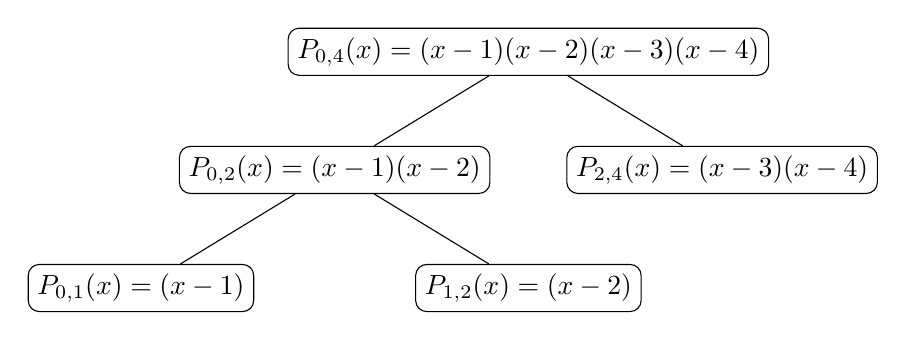
\begin{tikzpicture}[sibling distance=14em,
                every node/.style = {shape=rectangle, rounded corners,
                        draw, align=center
                    }]]
            \node {\(P_{0, 4}(x) = (x - 1)(x - 2)(x - 3)(x - 4)\)}
            child { node {\(P_{0, 2}(x) = (x - 1)(x - 2)\)}
                    child { node {\(P_{0, 1}(x) = (x - 1)\)}}
                    child { node {\(P_{1, 2}(x) = (x - 2)\)}}
                }
            child { node {\(P_{2, 4}(x) = (x - 3)(x - 4)\)}};
        \end{tikzpicture}
    \end{center}

    \pause

    \begin{itemize}
        \item Leaf 노드에서 올라가면서 다항식을 곱하자! \pause
        \item 트리 구성에 들어가는 비용
        \begin{itemize}
            \item 두 subtree\,의 root\,를 곱하는 비용 \(\O(n \log n)\) (FFT)
            \item 왼쪽, 오른쪽 subtree\,는 차수가 절반이므로 각각 \(T\left(\dfrac{n}{2}\right)\) \pause
        \end{itemize}
        \item \(T(n) = \ds 2 T\left(\frac{n}{2}\right) + \O(n \log n) \implies T(n) \in \alert{\O(n\log^2 n)}\)
    \end{itemize}
\end{frame}

\begin{frame}
    \frametitle{Polynomial Tree}
    \begin{center}
        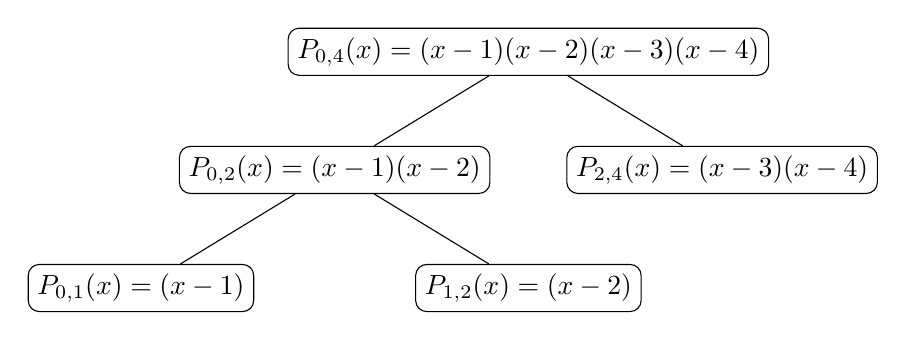
\begin{tikzpicture}[sibling distance=14em,
                every node/.style = {shape=rectangle, rounded corners,
                        draw, align=center
                    }]]
            \node {\(P_{0, 4}(x) = (x - 1)(x - 2)(x - 3)(x - 4)\)}
            child { node {\(P_{0, 2}(x) = (x - 1)(x - 2)\)}
                    child { node {\(P_{0, 1}(x) = (x - 1)\)}}
                    child { node {\(P_{1, 2}(x) = (x - 2)\)}}
                }
            child { node {\(P_{2, 4}(x) = (x - 3)(x - 4)\)}};
        \end{tikzpicture}
    \end{center}

    \begin{itemize}
        \item<1-> Root 노드에서 시작하여 \(f(x) \pmod{P_{l, r}(x)}\) 계산
        \item<2-> 계산 결과를 노드에 저장하고 결과를 subtree\,로 가져가 재귀 호출
        \item<3-> Leaf\,까지 내려오면 \(f(x_i)\)\,가 구해져 있음
    \end{itemize}
\end{frame}

\begin{frame}
    \frametitle{Polynomial Tree}
    \begin{center}
        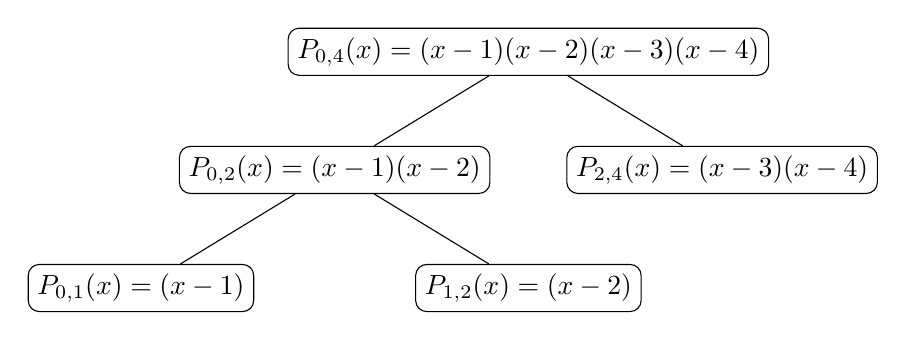
\begin{tikzpicture}[sibling distance=14em,
                every node/.style = {shape=rectangle, rounded corners,
                        draw, align=center
                    }]]
            \node {\(P_{0, 4}(x) = (x - 1)(x - 2)(x - 3)(x - 4)\)}
            child { node {\(P_{0, 2}(x) = (x - 1)(x - 2)\)}
                    child { node {\(P_{0, 1}(x) = (x - 1)\)}}
                    child { node {\(P_{1, 2}(x) = (x - 2)\)}}
                }
            child { node {\(P_{2, 4}(x) = (x - 3)(x - 4)\)}};
        \end{tikzpicture}
    \end{center}

    \begin{itemize}
        \item<1-> 최종 시간 복잡도
        \begin{itemize}
            \item<2-> 현재 노드에서 \(P_{l, r}(x)\)\,로 나누는데 걸린 시간 \(\O(n\log n)\)
            \item<3-> 왼쪽, 오른쪽 subtree\,는 차수가 절반이 되므로 각각 \(T\left(\dfrac{n}{2}\right)\)
        \end{itemize}
        \item<4-> \(T(n) = 2T\left(\dfrac{n}{2}\right) + \O(n\log n) \implies T(n) \in \alert{\O(n \log^2 n)}\)
    \end{itemize}
\end{frame}


\begin{frame}
    \frametitle{참고}
    \begin{itemize}
        \item DFT\,에서 \(\omega\inv\), Inverse DFT\,에서 \(\omega\)\,를 사용하기도 합니다.
        \item DFT Matrix\,를 unitary 행렬로 만들기 위해 \(1/\sqrt{n}\)\,으로 나누어서 사용하기도 합니다.
        \[
            W = \left(\frac{\omega^{ij}}{\sqrt{n}}\right)_{n \times n} \qquad W\inv = \left(\frac{\omega^{-ij}}{\sqrt{n}}\right)_{n \times n}
        \]
        단, NTT\,와 같이 다루는 집합에 따라 \(1/\sqrt{n}\)\,이 무의미한 경우도 있습니다.
        \item NTT\,의 일반적인 형태는 \href{https://en.wikipedia.org/wiki/Discrete_Fourier_transform_over_a_ring}{DFT Over a Ring}\,입니다.
        \item \(\omega\)\,가 아니라 임의의 복소수 \(z\)\,의 거듭제곱에서의 함숫값이 필요하다면 \href{https://en.wikipedia.org/wiki/Chirp_Z-transform}{Chirp \(Z\)-Transform}\,을 사용합니다.
    \end{itemize}
\end{frame}


\frame{\titlepage}

\end{document}
